% This is a general template file for the LaTeX package SVJour3
% for Springer journals. Original by Springer Heidelberg, 2010/09/16
%
% Use it as the basis for your article. Delete % signs as needed.
%
% This template includes a few options for different layouts and
% content for various journals. Please consult a previous issue of
% your journal as needed.
%
\RequirePackage{fix-cm}
%
%\documentclass{svjour3}                     % onecolumn (standard format)
%\documentclass[smallcondensed]{svjour3}     % onecolumn (ditto)
\documentclass[smallextended]{svjour3}       % onecolumn (second format)
%\documentclass[twocolumn]{svjour3}          % twocolumn
%
\smartqed  % flush right qed marks, e.g. at end of proof
%
\usepackage{graphicx}
\usepackage{amssymb}

\usepackage{caption}
\usepackage{subcaption}
%\usepackage{gnuplottex}
\usepackage{tikz}
\usepackage{mathtools}

\usepackage{graphicx}
\usepackage{hyperref}
\usepackage{textcomp}

\usepackage{algpseudocode}
\usepackage{algorithm}
\usepackage{algorithmicx}
\usepackage{verbatim}
%
% insert here the call for the packages your document requires
%\usepackage{mathptmx}      % use Times fonts if available on your TeX system
%\usepackage{latexsym}
% etc.
%
% please place your own definitions here and don't use \def but
% \newcommand{}{}
%
% Insert the name of "your journal" with
% \journalname{myjournal}
%
\begin{document}

\title{Title
\thanks{Supported by the Russian Science Foundation grant 18-11-00100.}
}
% Grants or other notes about the article that should go on the front
% page should be placed within the \thanks{} command in the title
% (and the %-sign in front of \thanks{} should be deleted)
%
% General acknowledgments should be placed at the end of the article.

\subtitle{Subtitile}

%\titlerunning{Short form of title}        % if too long for running head

\author{First Author         \and
        Second Author %etc.
}

%\authorrunning{Short form of author list} % if too long for running head

\institute{F. Author \at
              first address \\
              Tel.: +123-45-678910\\
              Fax: +123-45-678910\\
              \email{fauthor@example.com}           %  \\
%             \emph{Present address:} of F. Author  %  if needed
           \and
           S. Author \at
              second address
}

\date{Received: date / Accepted: date}
% The correct dates will be entered by the editor

\newtheorem{mytheorem}{Theorem}
%\newtheorem{lemma}{Lemma}
\newtheorem{mydef}{Definition}

\algrenewcommand\algorithmicindent{0.5em}
\algnewcommand\algorithmicswitch{\textbf{switch}}
\algnewcommand\algorithmiccase{\textbf{case}}
\algnewcommand\algorithmicassert{\texttt{assert}}
\algnewcommand\Assert[1]{\State \algorithmicassert(#1)}
% New "environments"
\algdef{SE}[SWITCH]{Switch}{EndSwitch}[1]{\algorithmicswitch\ #1\ \algorithmicdo}{\algorithmicend\ \algorithmicswitch}
\algdef{SE}[CASE]{Case}{EndCase}[1]{\algorithmiccase\ #1}{\algorithmicend\ \algorithmiccase}

\algtext*{EndSwitch}
\algtext*{EndCase}
\algtext*{EndWhile}% Remove "end while" text
\algtext*{EndIf}% Remove "end if" text
\algtext*{EndFor}% Remove "end for" text
\algtext*{EndFunction}% Remove "end function" text

\newif\ifboldnumber
\newcommand{\boldnext}{\global\boldnumbertrue}


\maketitle

\begin{abstract}
Insert your abstract here. Include keywords, PACS and mathematical
subject classification numbers as needed.
\keywords{First keyword \and Second keyword \and More}
% \PACS{PACS code1 \and PACS code2 \and more}
% \subclass{MSC code1 \and MSC code2 \and more}
\end{abstract}

\section{Introduction}
\label{section_intro}








\section{The Motivating Example}
\label{section_motivating}

In this section, we formulate the problem of context-free path query evaluation, using a small graph and the classical \emph{same-generation query}~\cite{FndDB}, which cannot be expressed using regular expressions.

Let us have a graph database or any other object, which can be represented as a graph. The same-generation query can be used for discovering a vertex similarity, for example, gene similarity~\cite{GraphQueryWithEarley}. For graph databases, the same-generation query is aimed at finding all the nodes at the same hierarchy level. The language, formed by the paths between such nodes, is not regular and corresponds to the language of matching parentheses. Hence, the query is formulated as a context-free grammar.

For example, let us have a small double-cyclic graph (see Figure~\ref{Example_Graph}). One of the cycles has three edges, labeled with $a$, and the other has two edges, labeled with $b$. Both cycles are connected via a shared node $0$.

\begin{figure}[h]
	\[
	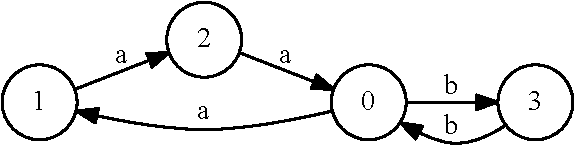
\includegraphics[width=7cm]{pictures/example_graph.pdf}
	\]
	\caption{An example graph.}
	\label{Example_Graph}
\end{figure}

For this graph, we have a same-generation query, formulated as a context-free grammar, which generates a context-free language \mbox{$L=\{a^n b^n~|~n \geq 1\}$}. This grammar is equal to $G = (N, \Sigma, P)$ where:
\begin{itemize}
	\item the set of non-terminals $N = \{S\}$;
	\item the set of terminals $\Sigma = \{a, b\}$;
	\item the set of production rules $P$ is presented on Figure~\ref{ProductionRulesWorsCaseExample}.
\end{itemize}

\begin{figure}[h]
	\[
	\begin{array}{rccl}
	0: & S & \rightarrow & \text{\emph{a}} \ S \ \text{\emph{b}} \\
	1: & S & \rightarrow & \text{\emph{a}} \ \text{\emph{b}} \\ 
	\end{array}
	\]
	\caption{Production rules for the example query grammar.}
	\label{ProductionRulesWorsCaseExample}
\end{figure}

Since our matrix-based algorithms for CFPQ processes only grammars in Chomsky normal form, we first transform the grammar $G$ into an equivalent grammar $G' = (N', \Sigma', P')$ in normal form, where:
\begin{itemize}
	\item the set of non-terminals $N' = \{S, S_1, A, B\}$;
	\item the set of terminals $\Sigma' = \{a, b\}$;
	\item the set of production rules $P'$ is presented on Figure~\ref{ProductionRulesExampleQueryCNF}.
\end{itemize}

\begin{figure}[h]
	\[
	\begin{array}{rccl}
	0: & S & \rightarrow & A \ B \\
	1: & S & \rightarrow & A \ S_1 \\
	2: & S_1 & \rightarrow & S \ B \\
	3: & A & \rightarrow & \text{\emph{a}} \\ 
	4: & B & \rightarrow & \text{\emph{b}} \\ 
	\end{array}
	\]
	\caption{Production rules for the example query grammar in normal form.}
	\label{ProductionRulesExampleQueryCNF}
\end{figure}

The result of context-free path query evaluation w.r.t. the relational query semantics for this example is a set of node pairs \mbox{$(m, n)$}, such that there is a path from the node $m$ to the node $n$, whose labeling forms a word from the language $L$. For example, the node pair \mbox{$(0,0)$} must be in this set, since there is a path from the node $0$ to the node $0$, whose labeling forms a string \mbox{$w = aaaaaabbbbbb = a^6b^6 \in L$}.

The result of context-free path query evaluation w.r.t. the single-path query semantics also contains such a path for each node pair \mbox{$(m, n)$} returned after the context-free path query evaluation w.r.t the relational query semantics. For example, if we want to provide proof of the existence of such a path for the node pair \mbox{$(0,0)$}, the path from the node $0$ to the node $0$, whose labeling forms a string \mbox{$w = a^6b^6$} can be returned. 
\section{Preliminaries} \label{section_preliminaries}
In this section, we introduce the basic notions used throughout the paper.

Let $\Sigma$ be a finite set of edge labels. Define an \textit{edge-labeled directed graph} as a tuple $D = (V, E)$ with $V$ is a set of nodes and $E \subseteq V \times \Sigma \times V$ is a directed edge-relation.  For a path $\pi$ in a graph $D$ we denote $l(\pi)$ --- the unique word obtained by concatenating the labels of the edges along the path $\pi$. Also, we write $n \pi m$ to indicate that a path $\pi$ starts at node $n \in V$ and ends at node $m \in V$.

According to Hellings~\cite{hellingsRelational}, we deviate from the usual definition of a context-free grammar in \textit{Chomsky Normal Form}~\cite{chomsky} by not including a special start non-terminal, which will be specified in the queries to the graph. Since every context-free grammar can be transformed into an equivalent one in Chomsky Normal Form and checking that an empty string is in the language is trivial, then it is sufficient to only consider grammars of the following type. A \textit{context-free grammar} is 3-tuple $G = (N, \Sigma, P)$ where $N$ is a finite set of non-terminals, $\Sigma$ is a finite set of terminals, and $P$ is a finite set of productions of the following forms:

\begin{itemize}
    \item $A \rightarrow B C$, for $A,B,C \in N$,
    \item $A \rightarrow x$, for $A \in N$ and $x \in \Sigma$.   
\end{itemize}

Note that we omit the rules of the form $A \rightarrow \varepsilon$, where $\varepsilon$ denotes an empty string. This does not limit the applicability of further algorithms because checking that an empty string belongs to the context-free language in Chomsky normal form is trivial and only the empty paths $m \pi m$ correspond to an empty string $\varepsilon$.

We use the conventional notation $A \xrightarrow{*} w$ to denote that the string $w \in \Sigma^*$ can be derived from a non-terminal $A$ by some sequence of applying the production rules from $P$. The \textit{language} of a grammar $G = (N,\Sigma,P)$ with respect to a start non-terminal $S \in N$ is defined by $L(G_S) = \{w \in \Sigma^*~|~S \xrightarrow{*} w\}$.

For a given graph $D = (V, E)$ and a context-free grammar $G = (N, \Sigma, P)$, we define \textit{context-free relations} $R_A \subseteq V \times V$, for every $A \in N$, such that $R_A = \{(n,m)~|~\exists n \pi m~(l(\pi) \in L(G_A))\}$.

We define a binary operation on arbitrary subsets $N_1 , N_2$ of $N$ with respect to a context-free grammar $G = (N, \Sigma, P)$ as $N_1 \cdot N_2 = \{A~|~\exists B \in N_1, \exists C \in N_2 \text{ such that }(A \rightarrow B C) \in P\}.$

Using this binary operation as a multiplication on arbitrary subsets of $N$ and union of sets as an addition, we can define a \textit{matrix multiplication}, $a \cdot b = c$, where $a$ and $b$ are matrices of the suitable size that have subsets of $N$ as elements, as $c_{i,j} = \bigcup^{n}_{k=1}{a_{i,k} \cdot b_{k,j}}$.

We define the \textit{transitive closure} of a square matrix $a$ as $a^+ = a^{(1)} \cup a^{(2)} \cup \cdots$ where $a^{(i)} = a^{(i-1)} \cup (a^{(i-1)} \cdot a^{(i-1)})$, $i \ge 2$ and $a^{(1)} = a$.
\section{Related works} \label{section_related}
The regular language constrained path querying is widely used for graph analysis~\cite{abiteboul1997regular,fan2011adding,nole2016regular,reutter2017regular}.

There are a number of solutions~\cite{azimov2018context,hellingsRelational,GraphQueryWithEarley,RDF} for context-free path query evaluation w.r.t. the relational query semantics, which employ such parsing algorithms as CYK~\cite{kasami,younger} or Earley~\cite{Grune}. Other examples of path query semantics are \textit{single-path} and \textit{all-path query semantics}. The all-path query semantics requires presenting all possible paths from node $m$ to node $n$ whose labeling is derived from a nonterminal $A$ for all triples $(A, m, n)$ evaluated using the relational query semantics. While the single-path query semantics requires presenting only one such a path for all the node-pairs $(m, n)$. Hellings~\cite{hellingsPathQuerying} presented algorithms for the context-free path query evaluation using the single-path and the all-path query semantics. If a context-free path query w.r.t. the all-path query semantics is evaluated on cyclic graphs, then the query result can be an infinite set of paths. For this reason, in~\cite{hellingsPathQuerying}, annotated grammars are proposed as a possible solution.

In~\cite{GLL}, the algorithm for context-free path query evaluation w.r.t. the all-path query semantics is proposed. This algorithm is based on the generalized top-down parsing algorithm~---~GLL~\cite{scott2010gll}. This solution uses derivation trees for the result representation which is more native for grammar-based analysis. The algorithms in~\cite{GLL,hellingsPathQuerying} for the context-free path query evaluation w.r.t. the all-path query semantics can also be used for query evaluation using the relational and the single-path semantics.

Hellings~\cite{hellingsRelational} presented an algorithm for the context-free path query evaluation using the relational query semantics. According to Hellings, for a given graph $D = (V, E)$ and a grammar $G = (N, \Sigma, P)$ the context-free path query evaluation w.r.t. the relational query semantics reduces to a calculation of the context-free relations $R_A$. Thus, in this work, we focus on the calculation of conjunctive relations which are similar to the context-free relations.

There is an algorithm~\cite{zhang2017context} for path querying with linear conjunctive grammars and relational query semantics. These grammars have no more than one nonterminal in each conjunct of the rule. The possibility of creating an algorithm for path query evaluation w.r.t. conjunctive grammars of an arbitrary form is an open problem since the linear conjunctive grammars are known to be strictly less powerful than the arbitrary conjunctive grammars~\cite{okhotinConjAndBool}.
\section{GPU section}
\label{section_GPU}
\section{Relaxed Parsing of Regular Sets}

The input of the algorithm (see Algorithm~\ref{parsing}) is a reference grammar $G$ with alphabet of terminal symbols $T$ 
and a finite non-deterministic automaton $(Q, \Sigma, \delta, q_0, q_f)$ with a single start state $q_0$, single final state $q_f$ 
and no $\epsilon$-transitions, where $\Sigma \subseteq T$~--- alphabet of input symbols, $Q$~--- alphabet of states, 
$\delta$~--- transition relation. RNGLR parser tables and some accessory information (called $parserSource$ in pseudocode) 
are generated for the grammar $G$. 

The general idea of the algorithm is to traverse the automaton graph and sequentially construct GSS, similarly to RNGLR.
However, as we deal with a graph instead of a linear stream, the next symbol turns into the \emph{set of terminals} on the 
all outgoing edges of current vertex. This results in a a different semantics of pushing and reducing (see line~5, 
Algorithm~\ref{processVertex}, and lines~8 and~20, Algorithm~\ref{gss_construction}). We use queue $\mathcal Q$ to control the 
order of automaton graph vertices processing. Every time a new GSS vertex is added, all zero-reductions have to be performed 
and then new tokens have to be shifted, so a corresponging graph vertex has to be enqueueed for further processing. 
Addition of new GSS edge can produce reductions to handle, so the graph vertex at the tail of the added edge has 
also to be enqueueed (see Algorithm~\ref{gss_construction}). Reductions are applied along the paths in GSS, and if we add
a new edge to some tail vertex, which was already presented in GSS, we also have to recalculate all \emph{passing} reductions
(see \emph{applyPassingReductions} function in Algorithm~\ref{processVertex}).

Likewise RNGLR, we associate GSS vertices with positions in the input,
and, in our case, a position coinsides with some state of the input automaton. We construct some
inner data structure (referred to as inner graph) by copying input automaton graph and 
extending each its vertex with the following collections: 

\begin{itemize}
  \item \emph{processed}: GSS vertices, for which all the pushes were processed. 
   This set aggregates all GSS vertices, associated with inner graph vertex.
  \item \emph{unprocessed}: GSS vertices, for which all the pushes are to be processed. 
   This set is analogous to $\mathcal{Q}$ of original RNGLR.
  \item \emph{reductions}: a queue, which is analogous to $\mathcal{R}$ of original RNGLR: 
   all reductions to be processed.
  \item \emph{passingReductionsToHandle}: pairs of GSS vertex and GSS edge to apply 
   passing reductions along them.
\end{itemize}

Besides parser $state$ and $level$ (which is equal to the input automaton state), 
a collection of \emph{passing reductions} is stored in a GSS vertex. Passing reduction is a 
triplet $(startV, N, l)$, representing reductions, whose path contains given GSS vertex. 
This triplet is similar to one describing reduction, where $l$ is a remaining length of the path. 
Passing reductions are stored for every vertex of the path (except for the first and the last) 
during path search in \emph{makeReductions} function (see Algorithm~\ref{processVertex}).

We inherit SPPF construction from the original RNGLR; in our case, 
derivation trees for strings, accumulated along the paths of the input automaton 
graph, are merged. 

\begin{algorithm}[!ht]
\begin{algorithmic}[1]
\caption{Parsing algorithm}
\label{parsing}
\Function{parse}{$grammar, automaton$}
  \State{$inputGraph \gets$ construct inner graph representation of $automaton$}
  \State{$parserSource \gets$ generate RNGLR parser tables for $grammar$}
  \If{$inputGraph$ contains no edges}
    \If{$parserSource$ accepts empty input} {report success}
    \Else { report failure}
    \EndIf
  \Else
    \State{\Call{addVertex}{$inputGraph.startVertex, startState$}}
    \State{$\mathcal{Q}.Enqueue(inputGraph.startVertex)$}
    \While{$Q$ is not empty}
      \State{$v \gets \mathcal{Q}.Dequeue()$}
      \State{\Call{makeReductions}{$v$}}
      \State{\Call{push}{$v$}}
      \State{\Call{applyPassingReductions}{$v$}}
    \EndWhile
    \If{$v_f.level = q_f$ and $v_f.state$ is accepting} {report success}
    \Else { report failure}
    \EndIf
  \EndIf
\EndFunction
\end{algorithmic}
\end{algorithm}

\begin{algorithm}[!ht]
\begin{algorithmic}[1]
\caption{Single-vertex processing}
\label{processVertex}
\Function{push}{$innerGraphV$}
  \State{$\mathcal{U} \gets$ copy $innerGraphV.unprocessed$}
  \State{clear $innerGraphV.unprocessed$}
  \ForAll{$v_{h}$ in $\mathcal{U}$}  
    \ForAll{$e$ in outgoing edges of $innerGraphV$}
      \State{$push \gets$ calculate next state by $v_{h}.state$ and the token on $e$}
      \State{\Call{addEdge}{$v_{h}, e.Target, push, false$}}
      \State{add $v_{h}$ in $innerGraphV.processed$}
    \EndFor
  \EndFor
\EndFunction

\Function{makeReductions}{$innerGraphV$}
  \While{$innerGraphV.reductions$ is not empty}
    \State{$(startV, N, l) \gets innerGraphV.reductions.Dequeue()$}
    \State{find the set of vertices $\mathcal{X}$ reachable from $startV$}
    \State{along the path of length ($l-1$), or $0$ if $l=0$;}
    \State{add $(startV, N, l-i)$ in $v.passingReductions$,}
    \State{where $v$ is an $i$-th vertex of the path}
    \ForAll{$v_{h}$ in $\mathcal{X}$}
      \State{$state_{t} \gets$ calculate new state by $v_{h}.state$ and nonterminal $N$}
      \State{\Call{addEdge}{$v_{h}, startV, state_{t}, (l=0)$}}
    \EndFor
  \EndWhile
\EndFunction

\Function{applyPassingReductions}{$innerGraphV$}
  \ForAll{$(v, edge)$ in $innerGraphV.passingReductionsToHandle$}
    \ForAll{$(startV, N, l) \gets v.passingReductions.Dequeue()$}
      \State{find the set of vertices $\mathcal{X}$,}
      \State{reachable from $edge$ along the path of length ($l-1$)}
      \ForAll{$v_{h}$ in $\mathcal{X}$}
        \State{$state_{t} \gets$ calculate new state by $v_{h}.state$ and nonterminal $N$}
        \State{\Call{addEdge}{$v_{h}, startV, state_{t}, false$}}
      \EndFor
    \EndFor
  \EndFor
\EndFunction
\end{algorithmic}
\end{algorithm}
 
\begin{algorithm}[!ht]
\begin{algorithmic}[1]
\caption{GSS construction}
\label{gss_construction}
\Function{addVertex}{$innerGraphV, state$}
  \If{$innerGraphV.processed$ or $innerGraphV.unprocessed$ contains\\
    vertex $v$ with state = $state$ }
    \State{\Return{($v, false$)}}
  \Else
    \State{$v \gets$ create new vertex for $innerGraphV$ with state $state$}
    \State{add $v$ in $innerGraphV.unprocessed$}
    \ForAll{$e$ in outgoing edges of $innerGraphV$}
      \State{calculate the set of zero-reductions by $v$}
      \State{and the token on $e$ and add them in $innerGraphV.reductions$}
    \EndFor
    \State{\Return{$(v, true$)}}
  \EndIf
\EndFunction

\Function{addEdge}{$v_{h}, innerGraphV, state_{t}, isZeroReduction$}
  \State{$(v_{t}, isNew) \gets$ \Call{addVertex}{$innerGraphV, state_{t}$}}
  \If{GSS does not contain edge from $v_{t}$ to $v_{h}$}
    \State{$edge \gets$ create new edge from $v_{t}$ to $v_{h}$}
    \State{$\mathcal{Q}.Enqueue(innerGraphV)$}
    \If{not $isNew$ and $v_{t}.passingReductions.Count>0$}
      \State{add $(v_{t}, edge)$ in $innerGraphV.passingReductionsToHandle$}
    \EndIf
    \If{not $isZeroReduction$}
      \ForAll{$e$ in outgoing edges of $innerGraphV$}
        \State{calculate the set of reductions by $v$}
        \State{and the token on $e$ and add them in $innerGraphV.reductions$}
      \EndFor
    \EndIf
  \EndIf
\EndFunction
\end{algorithmic}
\end{algorithm}

We conclude this section by justification of termination and correctness of our algorithm.

\textsc{Theorem 1.}
\textit{Algorithm terminates for any input.}

\textsc{Proof.}
Each vertex of inner representation of the input finite automaton contains, at most, 
$N$ GSS vertices, where $N$ is a number of parser states. So, the total number of 
GSS vertices is, at most, $N\times n$, where $n$ is the number of vertices in the inner graph. 
Since GSS has no multi-edges, the number of its edges is $O((N\times n)^2)$. The algorithm 
dequeues vertex to be processed from $\mathcal Q$ in the each iteration of the 
main loop. Vertices are enqueued to $\mathcal Q$ only when a new edge is added to GSS. Since the number of 
GSS edges is finite, the algorithm always terminates. \qed

To prove correctness, we first introduce the following definition:

\textsc{Definition.} 
\emph{Correct tree} is an ordered tree with the following properties:
\begin{enumerate}
  \item The root is the start nonterminal of the grammar $G$.
  \item The leaf nodes are terminals of $G$. The sequence of the leaf nodes 
        corresponds to some path in the inner graph. 
  \item The interior nodes are nonterminals of $G$. All children of nonterminal 
        $N$ correspond to the symbols of the right-hand side of some production for $N$ in $G$.
\end{enumerate}

Informally, correct tree is a derivation tree (w.r.t reference grammar) for some word in 
the regular approximation. Now we have to prove, that SPPF contains only correct trees.

\textsc{Lemma.}
For every GSS edge $(v_{t}, v_{h})$, $v_{t} \in V_{t}.processed$, $v_{h} \in V_{h}.processed$, 
the terminals of the associated subtree correspond to some path in the inner graph $p$ 
from $V_{h}$ to $V_{t}$.

\textsc{Proof.}
The proof is by induction on the height of derivation tree. 
The base case is either some $\epsilon$-tree or a tree with the single leaf. An $\epsilon$-tree corresponds 
to a path of zero length; the tail and the head of the edge associated with $\epsilon$-tree are identical, 
thus the statement is true. A tree with the single leaf corresponds to a single terminal read from an edge 
($V_{h}$, $V_{t}$) of the inner graph, thus the statement is true.

A tree of height $k$ has a nonterminal $N$ as its root. By third statement of correct tree definition, 
there is a production $N \rightarrow A_{0}, A_{1}, \dots, A_{n}$ for children $A_{0}, A_{1}, \dots, A_{n}$ of the root node. 
A subtree $A_{i}$ is associated with GSS edge $(v_{t}^{i}, v_{h}^{i})$ and, as its height is $k-1$, by inductive hypothesis,
there is a path in the inner graph from $V_{h}^{i}$ to $V_{t}^{i}$. $V_{t}^i = V_{h}^{i+1}$, since $v_{t}^i = v_{h}^{i+1}$, 
thus there is a path in the inner graph from $V_{h}^{0}$ to $V_{t}^{n}$, corresponding to the tree under consideration.
\qed

\textsc{Theorem 2.} 
\textit{Every generated from SPPF tree is correct.}

\textsc{Proof.} Consider arbitrary tree, generated from SPPF, and prove that it is correct. The first and the third statements
of correctness definition immediately follow from SPPF definition. 

{\bf (did'not understand the following statement; Russian decryption is required:)}
\textsc{Lemma 1} proves the second item of the definition by consideration of all the edges from the GSS vertex
on the last level having accepting state to the vertex on the 0-level with the start parser state.

\qed

\textsc{Theorem 3.} 
\textit{For every path $p$ in the inner graph, a correct tree corresponding to $p$ can be generated from SPPF.}

\textsc{Proof.}
Consider arbitrary correct tree and show it can be generated from SPPF. The proof follows the proof of correctness 
for RNGLR-algorithm, except the following moment. RNGLR constructs GSS layer-by-layer: it is guaranteed, that $j$-th 
level of the GSS $\forall j \in [0..i-1]$ would be fixed by the time, when $i$-th level is processed. In our case, 
this property does not hold, which leads to possible generation of the paths for reductions already applied. 
The only possible way to actually add a new path is to add an edge $(v_{t}, v_{h})$, where $v_{t}$ is already in the GSS and 
it has incoming edges. Since the algorithm stores, which reductions have passed through each vertex, it is sufficient to 
{\bf (what does it mean: ``continue passing reductions?'')} continue passing reductions, stored in $v_{t}$ to overcome this problem, 
and this is exactly what \emph{applyPassingReductions} function does. 
\qed

\section{Evaluation}

We evaluate the implemented algorithm on both regular and context-free path queries in order to demonstrate applicability of the proposed solution.
Namely, goals of the evaluation are following.
\begin{enumerate}
	\item Investigate the practical applicability of RPQ evaluation by the proposed algorithm.
	\item Compare Azimov's algorithm for reachability CFPQ and the proposed algorithm.
	\item Investigate the practical applicability of paths extraction algorithm for both regular and context-free queries.
\end{enumerate}

For evaluation, we use a PC with Ubuntu 18.04 installed.
It has Intel core i7-6700 CPU, 3.4GHz, and DDR4 64Gb RAM.
As far as we evaluate only algorithm execution time, we store each graph fully in RAM as its adjacency matrix in sparse format.
Note, that graph loading time is not included in the result time of evaluation.	

\subsection{RPQ Evaluation}

In oder to investigate applicability of the proposed algorithm for RPQ over real-world graphs we collect a set of real-world and synthetic graphs and evaluate queries generated by using the most popular templates for RPQs.

\subsubsection{Dataset}

Brief description of collected graphs are presented in Table~\ref{tbl:graphs_for_rpq}.
Namely, the dataset consists of several parts.
The first one is a set of LUBM graphs\footnote{Lehigh University Benchmark (LUBM) web page: \url{http://swat.cse.lehigh.edu/projects/lubm/}. Access date: 07.07.2020.}~\cite{10.1016/j.websem.2005.06.005} with a different number of vertices.
The second one is a graphs from Uniprot database\footnote{Universal Protein Resource (UniProt) web page: \url{https://www.uniprot.org/}. All files used for evaluation can be downloaded here: \url{ftp://ftp.uniprot.org/pub/databases/uniprot/current_release/rdf/}. Access date: 07.07.2020.}: \textit{proteomes}, \textit{taxonomy} and \textit{uniprotkb}.
The last part is a RDF files \textit{mappingbased\_properties} from DBpedia\footnote{DBpedia project web site: \url{https://wiki.dbpedia.org/}. Access date: 07.07.2020.} and \textit{geospecies}\footnote{The Geospecies RDF: \url{https://old.datahub.io/dataset/geospecies}. Access date: 07.07.2020.}.
These graphs represent data from different areas and they are frequently used for graph querying algorithms evaluation.

\begin{table}
{
\rowcolors{2}{black!2}{black!10}
\begin{tabular}{|l|c|c|}
\hline
Graph & \#V & \#E \\
\hline
\hline 
LUBM1k  & 120 926 & 484 646 \\
LUBM3.5k  & 358 434 & 144 9711 \\
LUBM5.9k  & 596 760 & 2 416 513 \\
LUBM1M   & 1 188 340 & 4 820 728 \\
LUBM1.7M & 1 780 956 & 7 228 358 \\
LUBM2.3M & 2 308 385 & 9 369 511 \\
\hline
Uniprotkb & 6 442 630 & 24 465 430 \\
Proteomes & 4 834 262 & 12 366 973 \\
Taxonomy & 5 728 398 & 14 922 125 \\
\hline
Geospecies & 450 609 & 2 201 532 \\
Mappingbased\_properties & 8 332 233 & 25 346 359 \\
\hline
\end{tabular}
}
\caption{Graphs for RPQ evaluation}
\label{tbl:graphs_for_rpq}
\end{table}


Queries for evaluation was generated by using templates of the most popular RPQs which are collected from~
\cite{Pacaci2020RegularPQ} (Table 2) and~\cite{Wang2019} (some of complex queries from Table 5), and are presented in table~\ref{tbl:queries_templates}.
We generate 10 queries for each template and each graph using the most frequent relations from the given graph randomly\footnote{Used generator is available as part of CFPQ\_data project: \url{https://github.com/JetBrains-Research/CFPQ_Data/blob/master/tools/gen_RPQ/gen.py}. Access data: 07.07.2020.}. 
For all LUBM graphs common set of queries was generated in order to investigate scalability of the proposed algorithm.

\begin{table}
{\small
\renewcommand{\arraystretch}{1.25}
\rowcolors{2}{black!2}{black!10}
\begin{tabular}{|c|c||c|c|}
\hline

Name & Query & Name & Query \\
\hline
\hline 
$Q_1$   & $a^*$                               & $Q_9^5$    & $(a \mid b \mid c \mid d \mid e)^+$                     \\
$Q_2$   & $a\cdot b^*$                        & $Q_{10}^2$ & $(a \mid b) \cdot c^*$                                  \\
$Q_3$   & $a \cdot b^* \cdot c^*$             & $Q_{10}^3$ & $(a \mid b \mid c)  \cdot d^*$                          \\
$Q_4^2$ & $(a \mid b)^*$                      & $Q_{10}^4$ & $(a \mid b \mid c \mid d)  \cdot e^*$                   \\
$Q_4^3$ & $(a \mid b \mid c)^*$               & $Q_{10}^5$ & $(a \mid b \mid c \mid d \mid e)  \cdot f^*$            \\
$Q_4^4$ & $(a \mid b \mid c \mid d)^*$        & $Q_{10}^2$ & $a \cdot b$                                             \\
$Q_4^5$ & $(a \mid b \mid c \mid d \mid e)^*$ & $Q_{11}^3$ & $a \cdot b \cdot c$                                     \\
$Q_5$   & $a \cdot b^* \cdot c$               & $Q_{11}^4$ & $a \cdot b \cdot c \cdot d$                             \\
$Q_6$   & $a^* \cdot b^*$                     & $Q_{11}^5$ & $a \cdot b \cdot c \cdot d \cdot f$                     \\
$Q_7$   & $a \cdot b \cdot c^*$               & $Q_{12}$   & $(a \cdot b)^+ \mid  (c \cdot d)^+$                     \\
$Q_8$   & $a? \cdot b^*$                      & $Q_{13}$   & $(a \cdot(b \cdot c)^*)^+ \mid  (d \cdot f)^+$          \\
$Q_9^2$ & $(a \mid b)^+$                      & $Q_{14}$   & $(a \cdot b \cdot (c \cdot d)^*)^+  \cdot (e \mid f)^*$ \\
$Q_9^3$ & $(a \mid b \mid c)^+$               & $Q_{15}$   & $(a \mid b)^+ \cdot (c \mid d)^+$                       \\
$Q_9^4$ & $(a \mid b \mid c \mid d)^+$        & $Q_{16}$   & $a \cdot b \cdot (c \mid d \mid e)$                     \\
\hline
\end{tabular}
}
\caption{Queries' templates for RPQ evaluation}
\label{tbl:queries_templates}
\end{table}


\subsubsection{Results}

For reachability index creation average time of 5 runs is presented.

Reachability index creation time for each query for LUBM graphs set is presented in figure~\ref{fig:lubm_all_qs}.
We can observe linear !!!! dependency of evaluation time on graph size.
Also we can see, that query evaluation time depends on query: there are queries which evaluate less then 1 second even for biggest graph ($Q_2$, $Q_5$, $Q_{11}^2$, $Q_{11}^3$), while worst time is 6.26 seconds ($Q_{14}$).
Anyway, we can argue that in this case our algorithm demonstrates reasonable time to be applied for real-world data analysis, because it is comparable with recent results on the same problem for LUBM querying by using distributed system over 10 nodes~\cite{Wang2019}, while we use only one node. 
Note, that accurate comparison of different approaches is a huge interesting work for the future.

\begin{figure}
   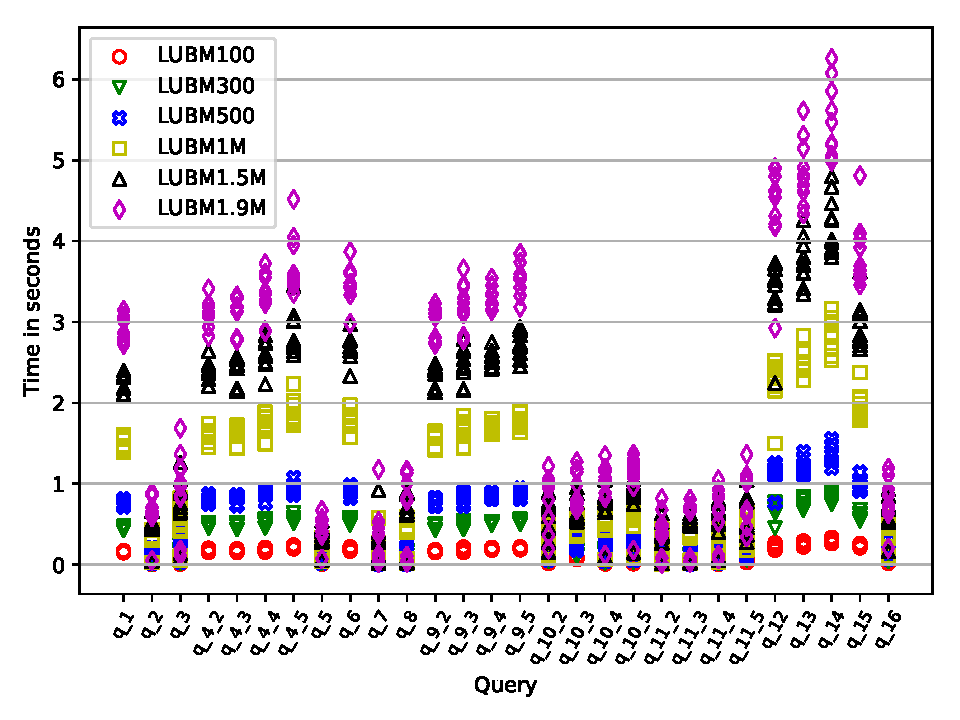
\includegraphics[width=0.48\textwidth]{data/LUBM_all.pdf}
   \caption{Reachability index creation time for LUBM graphs}
   \label{fig:lubm_all_qs}
\end{figure}

Reachability index creation time for each query for for real-world graphs is presented in figure~\ref{fig:other_all_qs}.
We can see that query evaluation time depends on graph inner structure. 
First of all, in some cases handling of small graph requires more time, then handling bigger graph.
For example, $Q_{10}^4$: querying the \textit{geospecies} graph (450k vertices) in some cases requires more time than querying of \textit{mappingbased\_properties} (8.3M vertices) and \textit{taxonomy} (5.7M vertices).
On the other hand, \textit{taxonomy} querying in relatively big number of cases requires significantly more time, than querying of other graphs, while \textit{taxonomy} is not a biggest graph. 
Finally, we can see, that in big number of cases query execution time requires less then 10 seconds, even for big graph, and no queries which require more then 52.17 seconds. 

\begin{figure}
   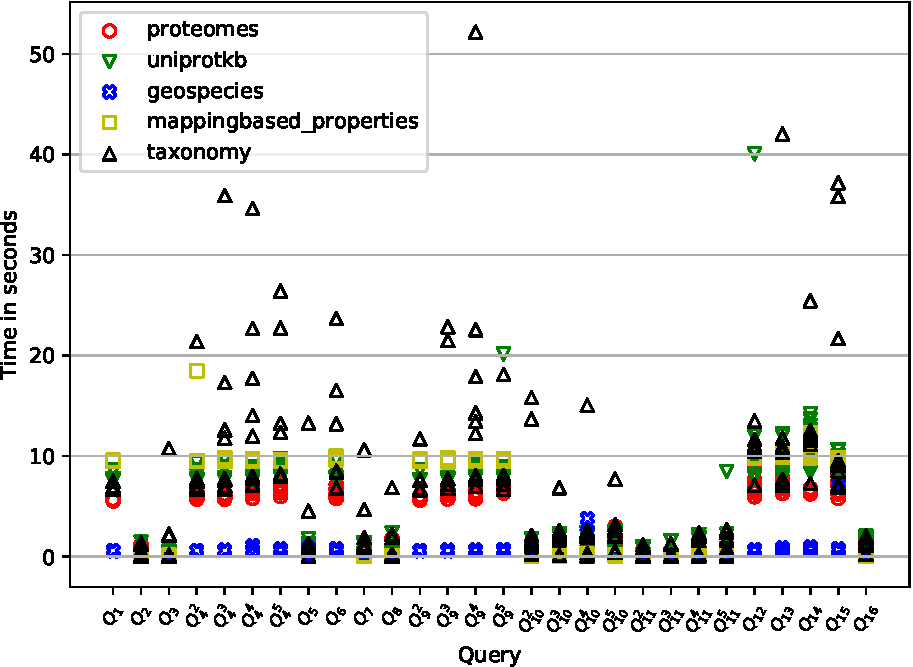
\includegraphics[width=0.48\textwidth]{data/other_all.pdf}
   \caption{Reachability index creation time for real-world RDFs}
   \label{fig:other_all_qs}
\end{figure}

Paths extraction was evaluated on cases with possible long paths.
These cases were selected during reachability index creation by using number of iterations in transitive closure evaluation.
For each selected graph and query we measure paths extraction time for each reachable pair, reachability index creation time is not included because exactly the same index, as calculated at the previous step, is used for paths extraction. 

We evaluate two scenarios.
The first one is a single path extraction.
In this case results are represented as a dependency of extraction time on extracted path length.
We can see linear !!!!

The second scenario is many paths extraction.
Here we limit a number of path to extract by !!! 
In this case results are represented as a dependency of extraction time on number of extracted paths.


\begin{figure}
     \begin{subfigure}[b]{0.24\textwidth}
         \centering
         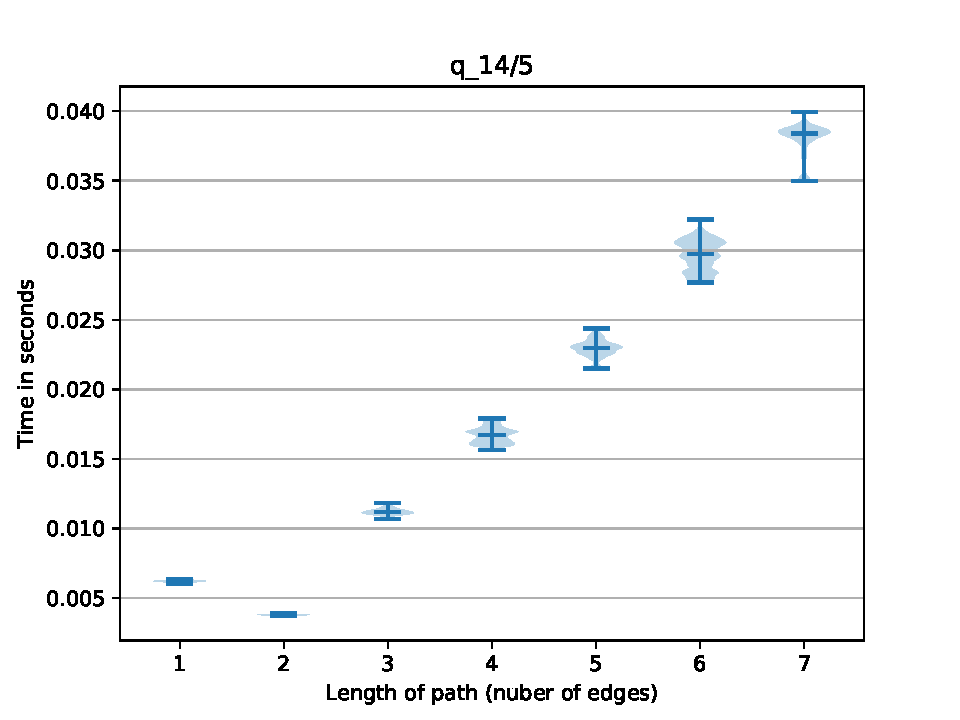
\includegraphics[width=\textwidth]{data/res_graphics/q_14_5.pdf}
         \caption{$y=x$}
         \label{fig:y equals x}
     \end{subfigure}
     ~\begin{subfigure}[b]{0.24\textwidth}
         \centering
         %\includegraphics[width=\textwidth]{data/res_graphics/q9_2_8.pdf}
         \caption{$y=x$}
         \label{fig:y equals x}
     \end{subfigure}\\
     \begin{subfigure}[b]{0.24\textwidth}
         \centering
         %\includegraphics[width=\textwidth]{data/res_graphics/q_14_8.pdf}
         \caption{$y=x$}
         \label{fig:y equals x}
     \end{subfigure}
     ~\begin{subfigure}[b]{0.24\textwidth}
         \centering
         %\includegraphics[width=\textwidth]{data/res_graphics/q4_2_8.pdf}
         \caption{$y=x$}
         \label{fig:y equals x}
     \end{subfigure}
   %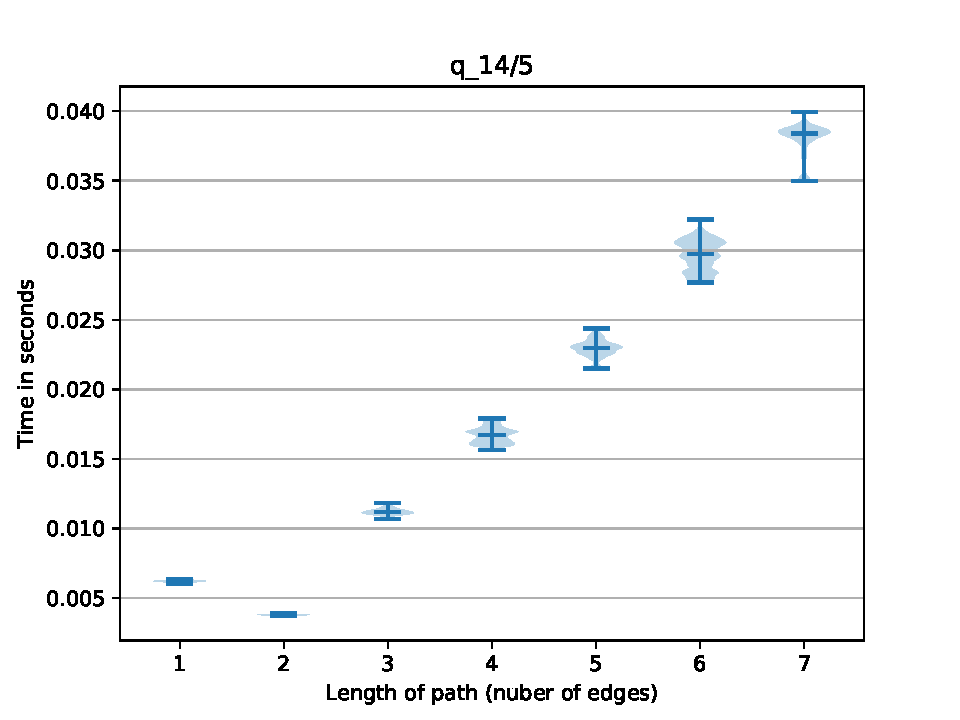
\includegraphics[width=0.48\textwidth]{data/res_graphics/q_14_5.pdf}
   \caption{Single path extraction}
\end{figure}

\subsubsection{Conclusion}

We can conclude that proposed algorithm is applicable for real-world data processing: the algorithm allows one both to solve reachability problem and to extract paths of interest in reasonable time even using na{\"i}ve implementation.  

\subsection{CFPQ Evaluation}

Comparison with matrix-based algorithm.

\subsubsection{Dataset}

Dataset for evaluation. 
It should be CFPQ\_Data\footnote{CFPQ\_Data is a dataset for CFPQ evaluation which contains both synthetic and real-world data and queries \url{https://github.com/JetBrains-Research/CFPQ\_Data}. Access date: 07.07.2020.}

\begin{table}
{
\rowcolors{2}{black!2}{black!10}
\begin{tabular}{|l|c|c|}
\hline
Graph & \#V & \#E \\
\hline
\hline 
eclass\_514en  & 120 926 & 484 646 \\
enzyme  & 358 434 & 144 9711 \\
geospecies  & 596 760 & 2 416 513 \\
go   & 1 188 340 & 4 820 728 \\
go-hierarchy & 1 780 956 & 7 228 358 \\
taxonomy & 2 308 385 & 9 369 511 \\
\hline
Aliases 1 & 6 442 630 & 24 465 430 \\
Aliases 2 & 4 834 262 & 12 366 973 \\
.... & 5 728 398 & 14 922 125 \\
\hline
\end{tabular}
}
\caption{Graphs for CFPQ evaluation}
\label{tbl:graphs_for_cfpq}
\end{table}



Same-generation queries, memory aliases.

\subsubsection{Results}

Results of evaluation.

Index creation.

{\setlength{\tabcolsep}{0.4em}
	\begin{table}
		\caption{RDFs query $G_1$ and $G_2$ (time is measured in seconds and memory is measured in megabytes)}
		\label{tbl:tableRDFQ1_appendix}
		\rowcolors{4}{black!2}{black!10}
		\small
		\begin{tabular}{| l | c | c | c | c |}
			\hline
			
			\multirow{2}{*}{Name}  & \multicolumn{2}{c|}{$G_1$} & \multicolumn{2}{c|}{$G_2$} \\
			\cline{2-5}
			                       & Tensors & RG\_CPU\textsubscript{path} & Tensors & RG\_CPU\textsubscript{path}	 \\
			\hline
			\hline
			eclass\_514en   & 0.254   & 0.195   & 0.227 & ...\\
			enzyme          & 0.035   & 0.029   & 0.036 & ...\\
			geospecies      & 0.091   & ...     & 0.001 & ...\\
			go-hierarchy    & 0.186   & 0.976   & 0.293 & ...\\
			go              & 1.676   & 1.286   & 1.368 & ...\\
			pathways        & 0.015   & 0.021   & 0.009 & ...\\
			taxonomy        & 5.366   & .....   & 3.282 & ...\\
			\hline
		\end{tabular}
	\end{table}
}


Paths extraction.

\subsubsection{Conclusion}

\section{Conclusion and future work}
In this paper, we shown how the context-free path query evaluation w.r.t. the relational and the single-path query semantics can be reduced to the calculation of matrix transitive closure. Also, we provided a formal proof of the correctness of the proposed reduction. In addition, we introduced an algorithm for computing this transitive closure, which allows us to efficiently apply GPGPU computing techniques. Finally, we shown the practical applicability of the proposed algorithm by running different implementations of our algorithm on real-world data.

We can identify several open problems for further research. In this paper we have considered only two semantics of context-free path querying but there are other important semantics, such as all-path query semantics~\cite{hellingsPathQuerying} which requires to present all paths for all triples $(A,m,n)$. Context-free path querying implemented with algorithm~\cite{GLL} can answer the queries in all-path query semantics by constructing a parse forest. It is possible to construct a parse forest for a linear input by matrix multiplication~\cite{okhotin_cyk}. Whether it is possible to generalize this approach for a graph input is an open question.

In our algorithm, we calculate the matrix transitive closure naively, but there are algorithms for the transitive closure calculation, which are asymptotically more efficient. Therefore, the question is whether it is possible to apply these algorithms for the matrix transitive closure calculation to the problem of context-free path querying.

Also, there are Boolean grammars~\cite{okhotinBoolean}, which have more expressive power than context-free grammars. Boolean path querying is an undecidable problem~\cite{hellingsRelational} but our algorithm can be trivially generalized to work on boolean grammars because parsing with boolean grammars can be expressed by matrix multiplication~\cite{okhotin_cyk}. It is not clear what a result of our algorithm applied to Boolean grammars would look like. Our hypothesis is that it would produce the upper approximation of a solution.

From a practical point of view, matrix multiplication in the main loop of the proposed algorithm may be performed on different GPGPU independently. It can help to utilize the power of multi-GPU systems and increase the performance of context-free path querying.

There is an algorithm~\cite{apspGPU} for transitive closure calculation on directed graphs which generalized to handle graph sizes inherently larger then the DRAM memory available on the GPU. Therefore, the question is whether it is possible to apply this approach to the matrix transitive closure calculation in the problem of context-free path querying.


%\begin{acknowledgements}
%If you'd like to thank anyone, place your comments here
%and remove the percent signs.
%\end{acknowledgements}

% BibTeX users please use one of
%\bibliographystyle{spbasic}      % basic style, author-year citations
%\bibliographystyle{spmpsci}      % mathematics and physical sciences
\bibliographystyle{spphys}       % APS-like style for physics
\bibliography{graphparsing}

\end{document}